\section{Factor investing and asset pricing anomalies}

Asset pricing anomalies are the foundations of factor investing. In this chapter our aim is twofold:
\begin{itemize}
    \item present simple ideas and concepts: basic factor models and common empirical facts
    \item provide a last of articles that go deeper on the topic.
\end{itemize}

This chapter is to create a broad overview of topics related to factor investing. For academically oriented studies look at \textit{Journal of Finance}, the \textit{Review of Financial Studies} and the \textit{Journal of Financial Economics}. For practitioner-oriented papers look at \textit{Journal of Portfolio Management} and the \textit{Financial Analysts Journal}.

\subsection{Introduction}
The core aim of factor models is to understand the \textbf{drivers of asset prices}.The rationale behind factor investing is that the \textit{financial performance of firms depends on factors, whether they be latent and unobservable, or related to intrinsic characteristics}. Cochrane (2011) frames the first essential question: \textit{which characteristics really provide independent information about average returns?}.

Linear factor models can be viewed as special cases of the arbitrage pricing theory (APT) of Ross (1976), which assumes that the return of an asset $n$ can be modelled as a linear combination of underlying factors $\boldsymbol{f_{k}}$:
\begin{equation}
    r_{t,n} = \alpha_{n} + \sum_{k=1}^{K} \beta_{n,k} \boldsymbol{f}_{t,k} + \epsilon_{t,n}, \label{eq:3}
\end{equation}
where the usual constraints on linear models hold: $\mathbb{E}[\epsilon _{t,n}] = 0$, $\operatorname{cov}(\epsilon _{t,n}, \epsilon_{t,m}) = 0$ for $n \neq m$ and $\operatorname{cov}(\mathbf{f}_{n}, \mathbf{\epsilon}_{n}) = 0$. If such factors do not exist then they are in contradiction with CAPM, which is the corner stone model of asset pricing. According to CAPM the only driver of returns is the market portfolio. This explains why factors are also called '\textit{anomalies}'. Pesaran and Smith (2021), the authors define the strength of factors using the sum of squared $\beta _{n,k}$ (across firms).

The regression \eqref{eq:3} can be evaluated once (unconditionally) or sequentially over different time frames. In the latter case, the parameters (coefficient estimates) change and the models are thus called \textit{conditional}. Conditional models are more flexible because they acknowledge that the drivers of asset prices may not be constant.

\subsection{Detecting anomalies}

\subsubsection{Challenges}
A crucial step is to be able to identify an anomaly and the complexity of this task should not be underestimated. Many findings are not reproducible. Nevertheless, as is demonstrated by A. Y. Chen (2019), $p$-hacking alone cannot account for all the anomalies documented in the literature. One way to reduce the risk of spurious detection is to increase the hurdles, or to resort to multiple testing. Nevertheless, the large sample sizes used in finance may mechanically lead to very low $p$-values.

The destruction of factor premia may be due to herding and could be accelerated by the democratization of so-called smart-beta products (ETFs notably) that allow investors to directly invest in particular styles. The book mentions a lot of different challenges, that are not shown in these notes. 

\subsubsection{Simple portfolio sort}
This is the most common procedure and it is used by Farma and French. The idea is simple. On one date, 
\begin{enumerate}
    \item rank firms according to a particular criterion (e.g, size, book-to-market ratio);
    \item form $J \geq 2$ portfolios (i.e. homogeneous groups) consisting of the same number of stocks according to the ranking (usually, $J=2$, $J=3$, $J=5$, or $J=10$ portfolios are built based on the median, terciles, quintiles or deciles of the criterion);
    \item the weight of stocks inside the portfolio is either uniform or proportional to market capitalization;
    \item at a future date (usually one month), report the returns of the portfolios. Then iterate the procedure until the chronological end of the sample is reached. 
\end{enumerate}

The outcome is a time series of portfolio returns $r_{t}^{j}$ for each grouping $j$. An anomaly is identified if the $t$-test between the first ($j=1$) and the last group ($j=J$) unveils a significant difference in average returns.  A strong limitation of this approach is that the sorting criterion could have a non-monotonic impact on returns and a test based on the two extreme portfolios would not detect it. Another concern is that these sorted portfolios may capture not only the priced risk associated to the characteristic, but also some unpriced risk.

Instead of focusing on only one criterion, it is possible to group asset according to more characteristics. The original paper (\textit{Fama and French (1992)}) also combines market capitalization with book-to-market ratios. Each characteristic is divided into 10 buckets, which makes 100 portfolios in total. There is no upper bound on the amount of features that can be included.

Olivier Ledoit, Wolf, and Zhao (2020) take into account the covariance structure of asset returns and to Cattaneo et al. (2020) for a theoretical study on the statistical properties of the sorting procedure (\textit{including theoretical links with regression-based approaches}). Notably, the latter paper discusses the optimal number of portfolios and suggests that it is probably larger than the usual 10 often used in the literature.

In the code below size portfolios are computes (equally weighted: above versus below the median capitalization). According to the size anomaly\footnote{Size anomaly: smaller companies (measured by market capitalization) tend to generate higher average returns compared to large companies over the long term.}, firms with below median market cap should earn higher returns on average. This is verified when the orange bar in the plot is above the blue one:

\begin{lstlisting}
data_ml |> 
    group_by(date) |> 
    mutate(large = Mkt_Cap_12M_Usd > median(Mkt_Cap_12M_Usd)) |> 
    ungroup() |> 
    mutate(year = lubridate::year(date)) |> 
    group_by(year, large) |> 
    summarise(avg_return = mean(R1M_Usd)) |> 
    ggplot(aes(x = year, y = avg_return, fill = large)) + 
    geom_col(position = "dodge") + 
    scale_fill_manual(values = c("#F8766D", "#619CFF"), labels = c("Small", "Large"), name = "") + 
    ylab("Average returns") +
    theme_minimal()
\end{lstlisting}

This gives the following histogram, which confirms the size anomaly (i.e., smaller companies tend to yield higher returns over time)
\begin{figure}[H]
    \caption{Size anomaly plot}
    \centering
    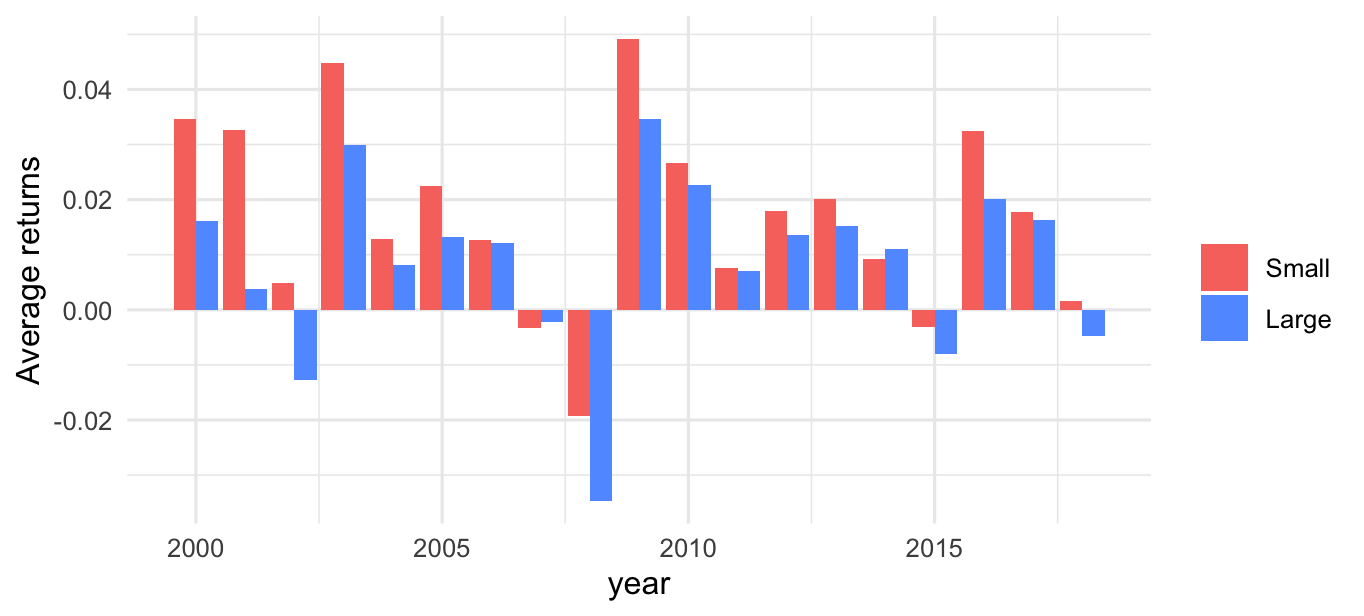
\includegraphics[width=0.75\textwidth]{part_1/images/size_anomaly.png}
\end{figure}


\subsubsection{Factors}
Factors are constructed like done above. Portfolios are based on one characteristic and the factor is a long-short ensemble of one extreme portfolio minus the opposite extreme (\textit{e.g., small minus large for the size factor or high book-to-market ratio minus large book-to-market-ratio for the value factor}). Sometimes, subtleties include forming bivariate sorts and aggregating several portfolios together. 

The most common factors are listed below, along with a few references. Look at the books listed at the beginning of the chapter for a more exhaustive treatment of factor idiosyncrasies.
\begin{itemize}
    \item Size (\textbf{SMB}): small firms minus large firms.
    \item Value (\textbf{HML}): high minus low: undervalues minus 'growth' firms.
    \item Momentum (\textbf{WML}): winners minus losers.
    \item Profitability (\textbf{RMW}): robust minus weak profits.
    \item Investment (\textbf{CMA}): conservative minus aggressive.
    \item Low 'risk' (\textbf{BAB}): betting against beta.
\end{itemize}

With the notable exception of the low risk premium, the most mainstream anomalies are kept and updated in the data library of Kenneth French (\href{https://mba.tuck.dartmouth.edu/pages/faculty/ken.french/data_library.html}{Dartmouth data library}). The computation of these factors follows a set of rules. Another source for data is the AQR repo: \href{https://www.aqr.com/Insights/Datasets}{AQR repository}.

These notes use a proxy for the value anomaly (\textit{I use not the book-to-market ratio, but price-to-book ratio}).

Below data from Ken French's data library is imported.
\begin{lstlisting}
min_date <- "1963-07-31"                  # Start date
max_date <- "2020-03-28"                  # Stop date

# Get KF data file of factors
temp <- tempfile()
KF_website <- "http://mba.tuck.dartmouth.edu/pages/faculty/ken.french/"
KF_file <- "ftp/F-F_Research_Data_5_Factors_2x3_CSV.zip"
link <- paste0(KF_website, KF_file)       # Link to file
download.file(link, temp, quiet = TRUE)   # Download file

# Clean up dataframe 
FF_factors <- read_csv(unz(temp, "F-F_Research_Data_5_Factors_2x3.csv"), skip = 3) |> 
  rename(date = '...1', MKT_RF = 'Mkt-RF') |> 
  mutate_at(vars(-date), as.numeric) |> 
  mutate(date = ymd(parse_date_time(date, "%Y%m"))) |> 
  mutate(date = rollback(date + months(1)))

# Scale returns
FF_factors <- FF_factors |> 
  mutate(
    MKT_RF = MKT_RF/100,
    SMB = SMB / 100,
    HML = HML / 100,
    RMW = RMW / 100,
    CMA = CMA / 100,
    RF = RF/100) |> 
  filter(date >= min_date, date <= max_date)
\end{lstlisting}

The six factors used by Farma and French can be seem below as they have been imported form Ken French's website:
\begin{table}[H]
    \centering
    \begin{tabular}[t]{lrrrrrr}
    \toprule
    date & MKT\_RF & SMB & HML & RMW & CMA & RF\\
    \midrule
    1963-07-31 & -0.0039 & -0.0041 & -0.0097 & 0.0068 & -0.0118 & 0.0027\\
    1963-08-31 & 0.0507 & -0.0080 & 0.0180 & 0.0036 & -0.0035 & 0.0025\\
    1963-09-30 & -0.0157 & -0.0052 & 0.0013 & -0.0071 & 0.0029 & 0.0027\\
    1963-10-31 & 0.0253 & -0.0139 & -0.0010 & 0.0280 & -0.0201 & 0.0029\\
    1963-11-30 & -0.0085 & -0.0088 & 0.0175 & -0.0051 & 0.0224 & 0.0027\\
    1963-12-31 & 0.0183 & -0.0210 & -0.0002 & 0.0003 & -0.0007 & 0.0029\\
    \bottomrule
    \end{tabular}
\end{table}

While these factors (i.e., long-short portfolios) exhibit time-varying risk premia and are magnified by corporate news and announcements, it is well-documented (and accepted) that they deliver positive returns over long horizons. it is well-documented (and accepted) that they deliver positive returns over long horizons and estimation methods can be improved.

Below we plot the average monthly return aggregated over each calendar year for five common factors. The risk free rate (which is not a factor per se) is the most stable, while the market factor (aggregate market returns minus the risk-free rate) is the most volatile. This makes sense because it is the only long equity factor among the five series.
\begin{lstlisting}
FF_factors |> 
  mutate(date = year(date)) |> 
  gather(key = factor, value = value, -date) |> 
  group_by(date, factor) |> 
  summarise(value = mean(value)) |> 
  ggplot(aes(x = date, y = value, color = factor)) + 
  geom_line() + 
  coord_fixed(200) + 
  theme_minimal()
\end{lstlisting}
\begin{figure}[H]
    \centering
    \caption{Average returns of common anomalies}
    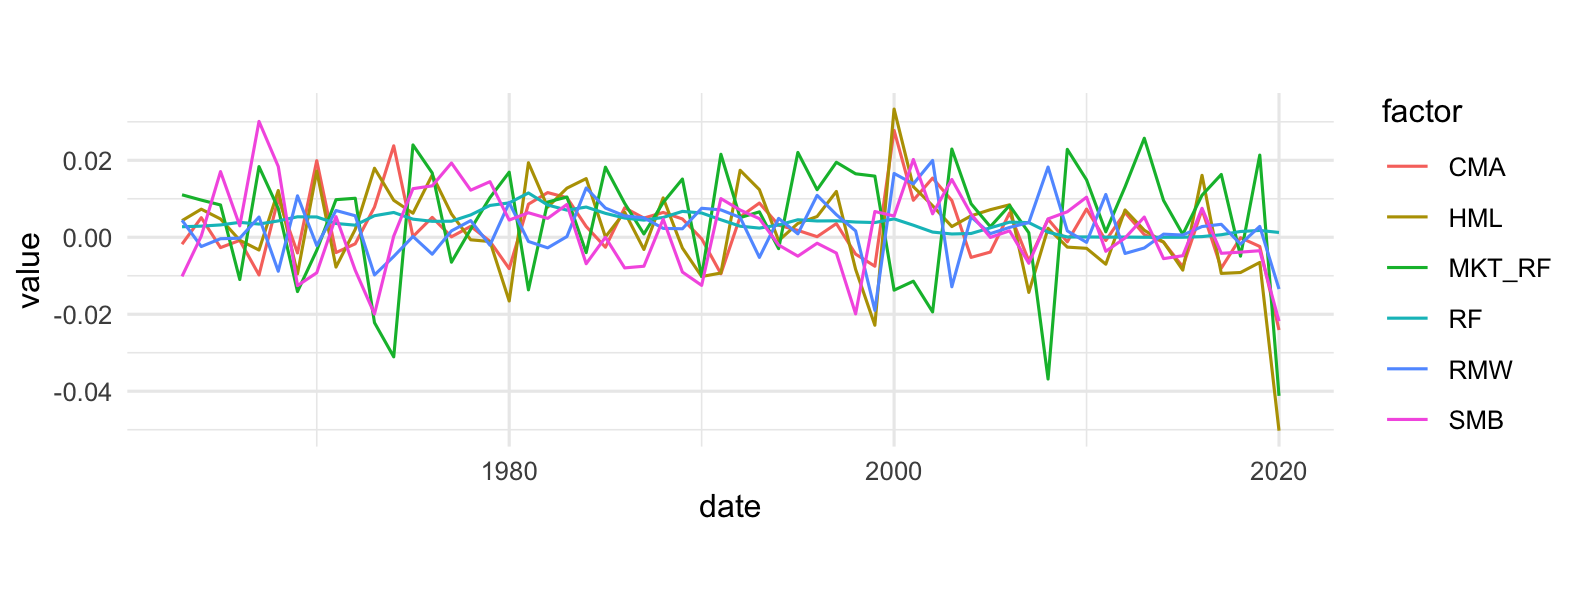
\includegraphics[width=0.85\textwidth]{part_1/images/factor_vals.png}
\end{figure}

As is shown by Linnainmaa and Roberts (2018) and Hou, Xue, and Zhang (2020), many proclaimed factors are in fact very much data-dependent and often fail to deliver sustained profitability when the investment universe is altered or when the definition of variable changes. Campbell Harvey and his co-authors, in a series of papers, tried to synthesize the research on factors in C. R. Harvey, Liu, and Zhu (2016), C. Harvey and Liu (2019) and C. R. Harvey and Liu (2019). His work underlines the need to set high bars for an anomaly to be called a \textit{true} factor. Increasing thresholds for $p$-values is only a partial answer, as it is always possible to resort to data snooping in order to find an optimized strategy that will fail out-of-sample but that will deliver a $t$-statistic larger than three (or even four). C. R. Harvey (2017) recommends to resort to a Bayesian approach which blends data-based significance with a prior into a so-called Bayesianized $p$-value.

Bryzgalova, Huang, and Julliard (2019) propose a tractable Bayesian estimation of large-dimensional factor models and evaluate all possible combinations of more than 50 factors, yielding an incredibly large number of coefficients. This combined with a Bayesianized Fama and MacBeth (1973) procedure allows to distinguish between pervasive and superfluous factors. Chordia, Goyal, and Saretto (2020) use simulations of 2 million trading strategies to estimate the rate of \textit{false discoveries}, that is, when a spurious factor is detected (type I error). They also advise to use thresholds for t-statistics that are well above three. In a similar vein, C. R. Harvey and Liu (2020) also underline that sometimes true anomalies may be missed because of a one time $t$-statistic that is too low (type II error).

The propensity of journals to publish positive results has led researchers to estimate the difference between reported returns and true returns. A. Y. Chen and Zimmermann (2020) call this difference the publication bias and estimate it as roughly 12\%. That is, if a published average return is 8\%, the actual value may in fact be closer to $(1-12\%)*8\%=7\%$. Qualitatively, this estimation of 12\% is smaller than the out-of-sample reduction in returns found in McLean and Pontiff (2016).

\subsubsection{Predective regressions, sorts, and $p$-value issues}
For simplicity, we assume a simple form:
\begin{equation}
    \mathbf{r} = a + b \mathbf{x} + \mathbf{e}
\end{equation}
where vector $\mathbf{r}$ stacks all returns of stocks and $\mathbf{x}$ is a lagged variable (\textit{regression is therefore predictive}). If $\hat{b}$ is significant given a specific threshold, then it can be tempting to conclude that $\mathbf{x}$ is a good predictor of returns. Hence, long-short portfolios related to extreme values of $\mathbf{x}$ are expected to to generate profits. This is not true, since $\hat{b}$ gives information on the past ability of $\mathbf{x}$ to forecast results. What is about to happen may be a different story.


Statistical tests are also used for portfolio sorts. Assume two extreme portfolios are expected to yield very different average returns. The portfolio returns are written as $r_{t}^{+}$ and $r_{t}^{-}$. The simplest test for the mean is $t = \sqrt{T}\frac{m_{r_{+}} - m_{r_{-}}}{\sigma_{r_{+} - r_{-}}}$, where $T$ is the number of points and $m_{r_{+}}$ denotes the means of returns and $\sigma _{r_{+} - r_{-}}$ is the standard deviation of the difference between the two series (\textit{i.e., volatility of the long-short portfolio}). The statistic can be viewed as a scaled Sharpe-ratio and can in turn be used to compute the $p$-values to assess the robustness of an anomaly. Many factors discovered by researchers fail to survive in out-of-sample tests.


One reason why people are overly optimistic about anomalies they detect is the widespread reverse interpretation of the $p$-value. Often, it is thought of as the probability of one hypothesis (\textit{e.g., my anomaly exists}) given the data. In fact, it's the opposite; it's the likelihood of your data sample, knowing that the anomaly holds.
\begin{align*}
    p & = P[D|H] \\
    \text{target prob} & = P[H|D]= \frac{P[D|H]}{P[D]} \cdot P[H]
\end{align*}
where $H$ standard for the hypothesis and $D$ for data. The equality in the second row is an application of Bayes' identity: the interesting probability is a transform of the $p$-value.

C. R. Harvey (2017) introduces Bayesianized $p$-values (Bpv)
\begin{equation*}
    \text{Bpv} = e^{ -\frac{t^{2}}{2} } \cdot \frac{\text{prior}}{1 + e^{ -\frac{t^{2}}{2} } \cdot \text{prior}}
\end{equation*}
where $t$ is the $t$-statistic from the regression (\textit{i.e., the one that defines the $p$-value}) and prior is the analyst's estimation of the odds that the hypothesis (anomaly) is true. The odds are coded as $p/(1-p)$. Thus, if the $t$-statistic is equal to 2 and the prior odds are equal to 6, then the Bpv is $e^{ -2 } \cdot 6 \cdot (1 + e^{ -2 } \cdot 6)^{-1} \approx 0.448$ and there is a $44.8\%$ chance the null is true. 

\subsubsection{Fama-McBeth regresssions}
Another detection method was proposed by Fama and MacBeth; two-stage regression analysis of risk prima. First step is a simple estimation of the relationship \eqref{eq:3}: the regressions are run on a stock-by-stock basis over corresponding time series. The resulting estimates $\hat{\beta}_{i,k}$ are plugged into a second series of regressions: 
\begin{equation*}
    r_{t,n} = \gamma _{t,0} + \sum _{k=1}^{K} \gamma _{t,k} \hat{\beta}_{n,k} + \varepsilon_{t,n}
\end{equation*}
which are run date-by-date on the cross-section of assets. Theoretically, the betas are known and the regression is run on $\beta _{n,k}$ instead of the estimated values. The $\hat{\gamma}_{t,k}$ estimate the premia of factor $k$ at time $t$. Under suitable distributional assumptions on $\varepsilon_{t,n}$, statistical test can be performed to determine whether these permia are significant or not. The statistical test most often used on the time-aggregated (average) premia $\hat{\gamma }_k = \frac{1}{T} \sum _{t=1}^{T} \hat{\gamma }_{t,k}$:
\begin{equation*}
    t_{k} = \frac{\hat{\gamma}_{k}}{\hat{\sigma}_{k}/\sqrt{T}} 
\end{equation*}
is often used in pure Gaussian contexts to assess whether or not the factor is significant ($\hat{\sigma }_k$ is the standard deviation of $\hat{\gamma}_{t,k}$).

Biases and losses in accuracy can be included by standard OLS estimations. Moreover, as the $\hat{\beta}_{i,k}$ in the second-pass regression are estimates, a second level of error can arise (called errors in variables). 

Below the Fama and MacBeth regressions are performed on our sample. We start by the first pass: individual estimation of betas. We build a dedicated function below and use some functional programming to automate the process. We stick to the original implementation of the estimation and perform synchronous regressions
\begin{lstlisting}
# Number of factors
nb_factors <- 5

# Create a dataframe with factors and all stock returns for a given date on each row
data_FM <- left_join(data_ml |> 
            dplyr::select(date, stock_id, R1M_Usd) |> 
            filter(stock_id %in% stock_ids_short), 
          FF_factors, 
          by = "date") |> 
  group_by(stock_id) |> 
  mutate(R1M_Usd = lag(R1M_Usd)) |> 
  ungroup() |> 
  na.omit() |> 
  pivot_wider(names_from = "stock_id", values_from = "R1M_Usd")

# Fit linear models of factors and returns over time for each stock 
models <- lapply(
  paste0("`", stock_ids_short, "`", " ~ MKT_RF + SMB + HML + RMW + CMA"), 
  function(f){ lm(as.formula(f), data = data_FM, na.action = "na.exclude") |> 
      summary() %>%
      "$"(coef) |> 
      data.frame() |> 
      dplyr::select(Estimate)}) 

# Format table of betas nicely
betas <- matrix(unlist(models), ncol = nb_factors + 1, byrow = TRUE) |> 
  data.frame(row.names = stock_ids_short)
colnames(betas) <- c("Constant", "MKT_RF", "SMB", "HML", "RMW", "CMA")
\end{lstlisting}

In the table below is a sample of the estimated betas for the first 6 stocks.
\begin{table}[H]
    \centering
    \begin{tabular}[t]{lrrrrrr}
    \toprule
      & Constant & MKT\_RF & SMB & HML & RMW & CMA\\
    \midrule
    1 & 0.0080073 & 1.4185896 & 0.5220226 & 0.6178794 & 0.9749334 & -0.3612393\\
    3 & -0.0022122 & 0.8115331 & 1.1048548 & 0.8853894 & 0.2972274 & -0.5544541\\
    4 & 0.0045092 & 0.3628417 & 0.3058171 & -0.0482520 & 0.5957859 & 0.1940631\\
    7 & 0.0053913 & 0.4310613 & 0.6745676 & 0.2316349 & 0.3212058 & 0.1723559\\
    9 & 0.0037773 & 0.8386114 & 0.6776150 & 1.0568940 & 0.0790805 & 0.0626698\\
    11 & -0.0011353 & 0.9842782 & 0.1179911 & 0.4887056 & -0.1288554 & 0.0112944\\
    \bottomrule
    \end{tabular}
\end{table}

Below we prepare the estimated betas for the second pass of regressions, where we bind the estimated factors for each stock to the stock returns of the same stock. 
\begin{lstlisting}
loadings <- betas |> 
  dplyr::select(-Constant) |> 
  data.frame()

ret <- returns |> 
  dplyr::select(-date) |> 
  data.frame(row.names = returns$date) |> 
  t()

FM_data <- cbind(loadings, ret)
\end{lstlisting}

We observe that the values of the first column (market betas) revolve around one, which is what we would expect. The second pass is done below, where try to estimate the effect of each factor on return of all stocks for a given date. We therefore get the factor prima for each day, which is how big the prima of each factor was every day.
\begin{lstlisting}
models <- lapply(
  paste("`", returns$date, "`", ' ~  MKT_RF + SMB + HML + RMW + CMA', sep = ""),
  function(f){ lm(as.formula(f), data = FM_data) |> 
      summary() %>%
      "$"(coef) |> 
      data.frame() |> 
      dplyr::select(Estimate)})

gammas <- matrix(unlist(models), ncol = nb_factors + 1, byrow = TRUE) |> 
  data.frame(row.names = returns$date)
colnames(gammas) <- c("Constant", "MKT_RF", "SMB", "HML", "RMW", "CMA") 

gammas[2:nrow(gammas),] |> 
  dplyr::select(MKT_RF, SMB, HML) %>% 
  bind_cols(date = data_FM$date) %>%
  gather(key = factor, value = gamma, -date) %>% 
  ggplot(aes(x = date, y = gamma, color = factor)) +
  geom_line() +
  facet_grid(factor ~.) + 
  theme_minimal()
\end{lstlisting}

Below is a plot showing the volatility of each market prima for factors over time. We observe that they are very volatile. 
\begin{figure}[H]
    \centering
    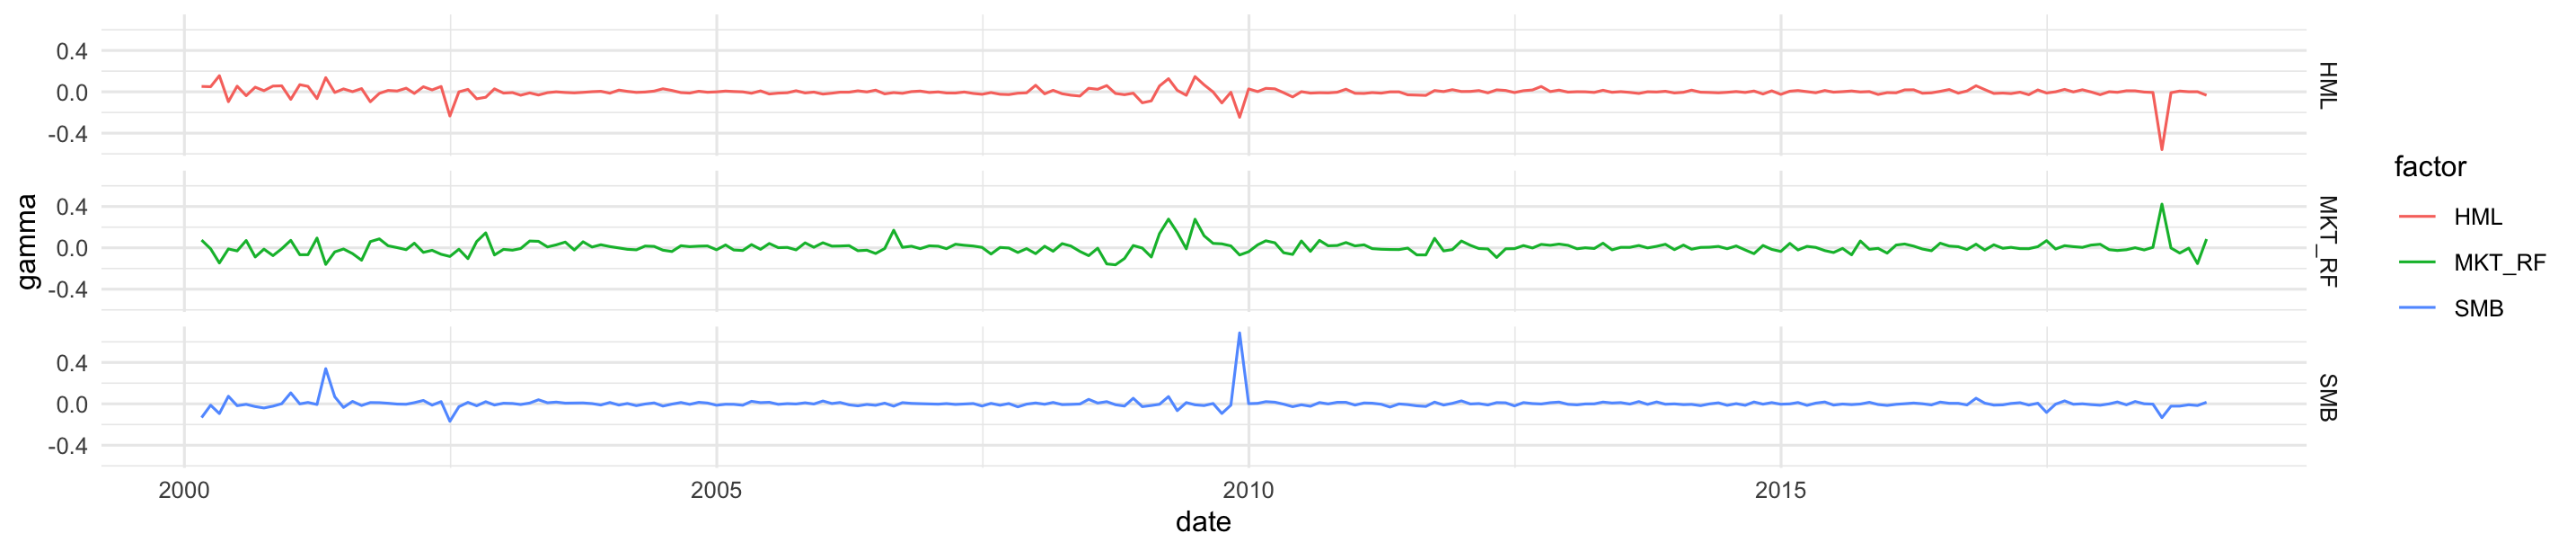
\includegraphics[width=0.95\textwidth]{part_1/images/factor_prima_markets.png}
\end{figure}

The two spikes at the end of the sample signal potential colinearity issues; two factors seem to compensate in an unclear aggregate effect. This underlines the usefulness of penalized estimates (discussed in later sections).

\subsubsection{Factor competition}
The core purpose of factors is to explain the cross-section of stock returns. For theoretical and practical reasons, it is preferable if redundancies within factors are avoided. Indeed, redundancies imply collinearity which is known to perturb estimates. In addition, when asset managers decompose the performance of their returns into factors, overlaps (high absolute correlations) between factors yield exposures that are less interpretable; positive and negative exposures compensate each other spuriously.

A simple protocol to sort out redundant factors is to run regressions of each factor against all others:
\begin{equation}
    f_{t,k} = a_{k} + \sum_{j \neq k} \delta_{k,j}f_{t,j} + \epsilon_{t,k} \label{eq:5}
\end{equation}
The metric of interest is the statistic associated with the estimation of $a_{k}$. If $a_{k}$ is significantly different from zero, then the cross-section of (other) factors fails to explain exhaustively the average return of factor. Otherwise, the return of the factor can be captured by exposures to the other factors and is thus redundant. In the regression above we try to estimate a factor for with all other factors. If we find that we need an additional terms to explain factor $k$ then they remaining factors fail to explain that factor $k$, i.e., that $k$ is not redundant; otherwise, we remaining factors $j \neq k$ can explain factor $k$ and thus imply redundancy.

One mainstream application of this technique was performed in Fama and French (2015), in which the authors show that the HML factor is redundant when taking into account four other factors (Market, SMB, RMW and CMA). This is shown below. 

We can run the regressions that determine the redundancy of factors via the procedure defined in \eqref{eq:5}.
\begin{lstlisting}
# All factors
factors <- c("MKT_RF", "SMB", "HML", "RMW", "CMA")

models <- lapply(
  paste(factors, ' ~ MKT_RF + SMB + HML + RMW + CMA - ', factors), 
  function(f){lm(as.formula(f), data = FF_factors) %>% 
      summary() %>% 
      "$"(coef) %>% 
      data.frame() %>% 
      filter(rownames(.) == "(Intercept)") %>% 
      dplyr::select(Estimate, `Pr...t..`)
    })

alphas <- matrix(unlist(models), ncol = 2, byrow = TRUE) %>% 
  data.frame(row.names = factors)
colnames(alphas) <- c("Estimate", "Signifcance")
alphas
\end{lstlisting}

This gives the following table of $\alpha$'s, where we can see that the factor HML is redundant when the four other factors are present in the pricing model. These results are close to those obtained in the study by Fama.
\begin{table}[H]
    \centering
    \begin{tabular}{lrr}
    \toprule
      & Estimate & Signifcance\\
    \midrule
    MKT\_RF & 0.0077969 & 0.0000004\\
    SMB & 0.0027418 & 0.0128758\\
    HML & -0.0005571 & 0.4884991\\
    RMW & 0.0038725 & 0.0000009\\
    CMA & 0.0023971 & 0.0000058\\
    \bottomrule
    \end{tabular}
\end{table}

Researchers also look at which factors maximize the likelihood of the observed data. Some papers seek to quantify to which extent the 3 factor model outperforms the 5 factor model.

\subsection{Hot topics: momentum, timing and ESG}

\subsubsection{Factor momentum}
A recent body of literature unveils a time series momentum property of factor returns. T. Gupta and Kelly (2019) report that autocorrelation patterns within these returns is statistically significant. Additional work points to the fact the industry momentum can be explained by factor momentum. In the extremes researches propose that the momentum factor is an aggregate of the autocorrelation found in all other factors\footnote{The strength of factor momentum has been scrutinized; the authors find that it is only robust for a small number of factors}.

H. Yang seeks to understand the source of factor momentum and decomposes stock factor momentum portfolios into two components: factor timing portfolio and a static portfolio. The former seeks to profit from the serial correlation of factor returns, whilst the latter tries to harness factor prima. The static portfolio explains a larger portion of factor momentum returns. H. Yang presents an estimator to gauge factor momentum predictability.

Given data obtained by Ken French, we compute the autocorrelation function of factors
\begin{equation*}
    \operatorname{ACF}_{k}(\mathbf{x}_{t}) = \mathbb{E}[(\mathbf{x}_{t} - \bar{\mathbf{x}})(\mathbf{x}_{t+k} - \bar{\mathbf{x}})]
\end{equation*}

\begin{lstlisting}
acf_SMB <- ggAcf(FF_factors$SMB, lag.max = 10) + labs(title = "") + theme_minimal()  # ACF SMB
acf_HML <- ggAcf(FF_factors$HML, lag.max = 10) + labs(title = "") + theme_minimal()  # ACF HML
acf_RMW <- ggAcf(FF_factors$RMW, lag.max = 10) + labs(title = "") + theme_minimal()  # ACF RMW
acf_CMA <- ggAcf(FF_factors$CMA, lag.max = 10) + labs(title = "") + theme_minimal()  # ACF CMA
plot_grid(acf_SMB, acf_HML, acf_RMW, acf_CMA,  # Plot
          labels = c('SMB', 'HML', 'RMW', 'CMA'))
\end{lstlisting}
which gives the following plots, where we observe that only the size factor is not significantly correlated at the first order.
\begin{figure}[H]
    \centering
    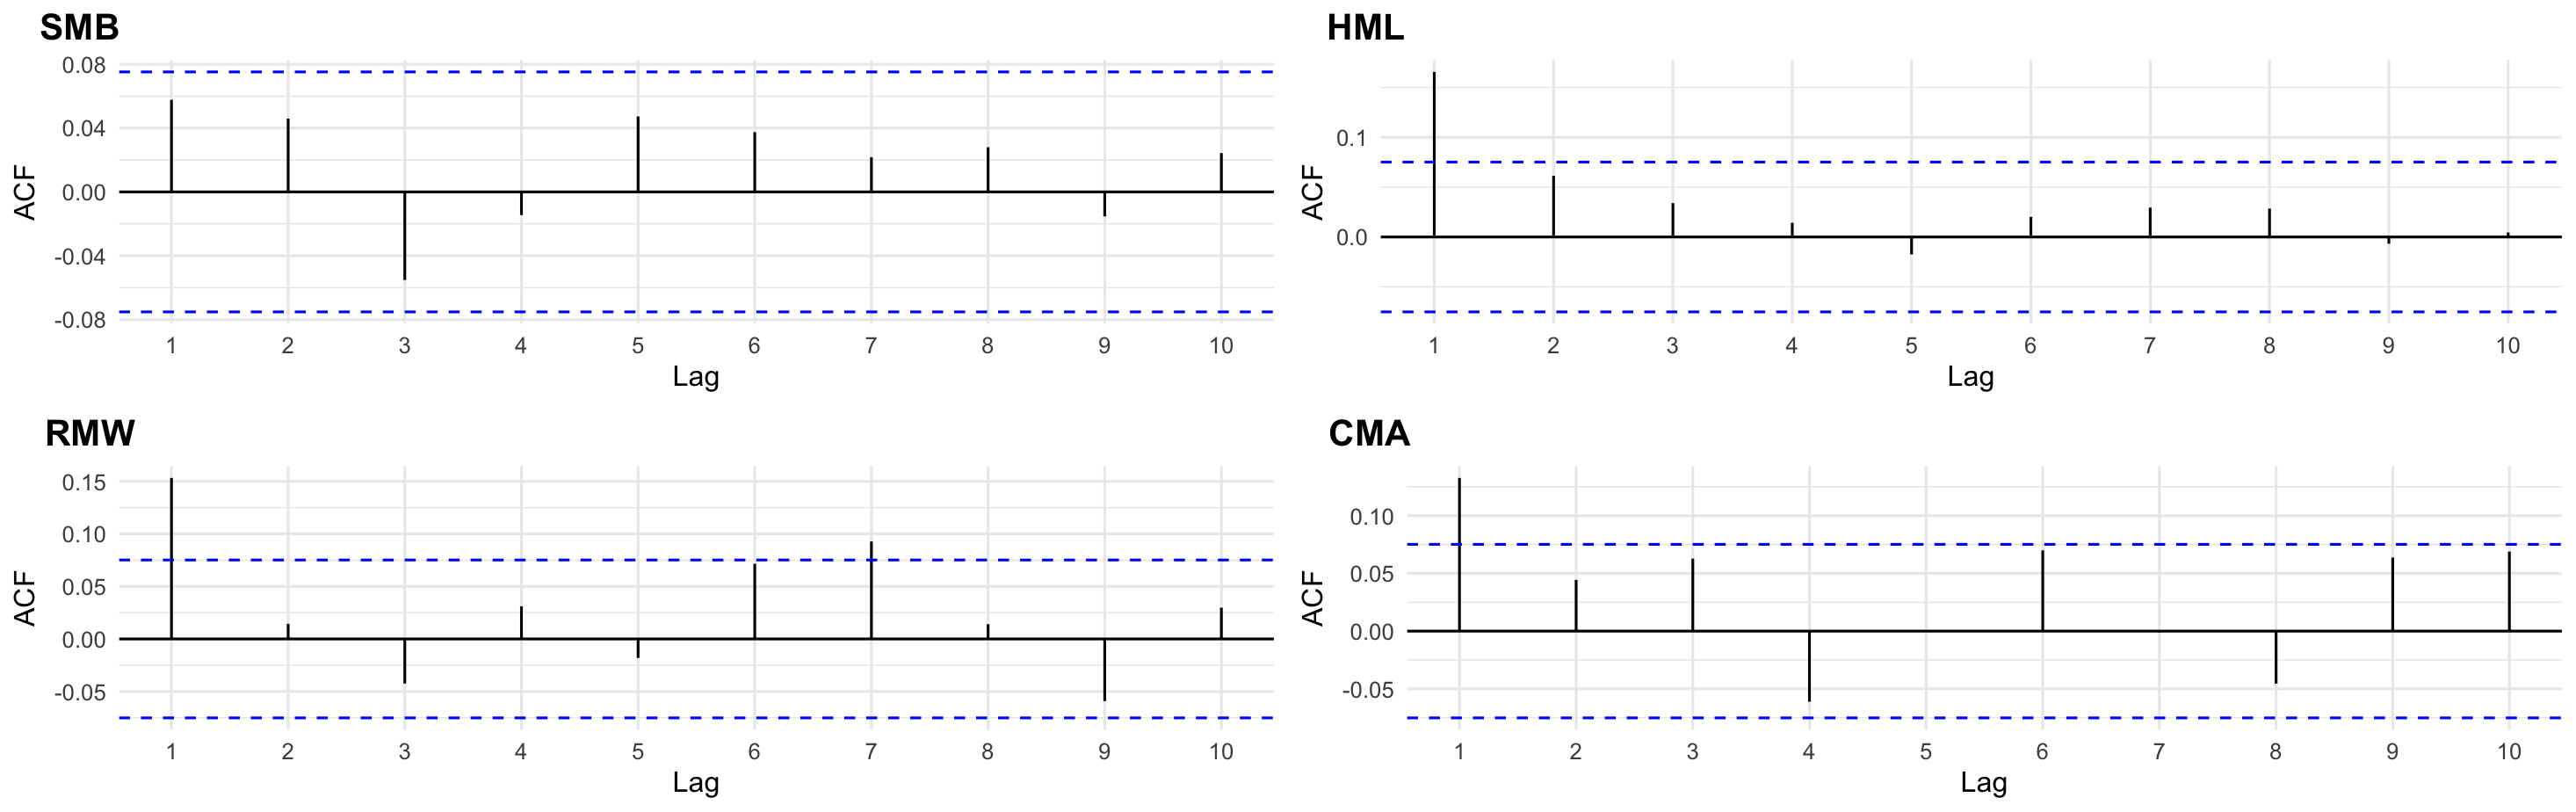
\includegraphics[width=\textwidth]{part_1/images/factor_autocorrelation.png}
\end{figure}

\subsubsection{Factor timing}
Given the abundance of evidence of the time-varying nature of factor premia, it is legitimate to wonder if it is possible to predict when factor will perform well or badly. The evidence on the effectiveness of timing is diverse. The majority of positive findings may be due to the bias towards positive results - but this is pure speculation.

There is no consensus on which predictors to use. A method for building reasonable timing strategies for long-only portfolios with sustainable transaction costs is laid out in Leippold and Rüegg (2020). The cross-section of characteristics is used for factor timing purposes in Kagkadis et al. (2021). In Vincenz and Zeissler (2021), it is found that macro variables are the best for this purpose. In ML-based factor investing, it is possible to resort to more granularity by combining firm-specific attributes to large-scale economic data.

\subsubsection{The green factors}

Demand for ethical financial products has risen lately. Not a new concept, but a lot more research has gone into if characteristics related to ESG criteria are priced or not (no consensus has been reached). Below are papers that suggest conflicting results:
\begin{itemize}[noitemsep]
    \item \textbf{Favorable}: ESG investing works (Kempf and Osthoff (2007), Cheema-Fox et al. (2020)), can work (Nagy, Kassam, and Lee (2016), Alessandrini and Jondeau (2020)), or can at least be rendered efficient (Branch and Cai (2012)). A large meta-study reports overwhelming favorable results (Friede, Busch, and Bassen (2015)), but of course, they could well stem from the publication bias towards positive results.
    \item \textbf{Unfavorable}: Ethical investing is not profitable according to Adler and Kritzman (2008) and Blitz and Swinkels (2020). An ESG factor should be long unethical firms and short ethical ones (Lioui (2018)).
    \item \textbf{Mixed}: ESG investing may be beneficial globally but not locally (Chakrabarti and Sen (2020)). Portfolios relying on ESG screening do not significantly outperform those with no screening but are subject to lower levels of volatility (Gibson et al. (2020), Gougler and Utz (2020)). As is often the case, the devil is in the details, and results depend on whether to use E, S or G (Bruder et al. (2019)).
\end{itemize}

ESG criteria can be directly integrated into a ML-model, as for instance done in France et al. (2020).

\subsection{Links with machine learning}
The task of linking alternative (\textit{e.g. sentiment data}) and traditional accounting data (\textit{e.g. accounting ratios}) is well suited for Machine Learning. Given a large set of predictor variables ($\mathbf{X}$), the goal is to predict a proxy for future performance $\mathbf{y}$ through a model of the firm discussed earlier
\begin{equation*}
    \mathbf{y} = f(\mathbf{X}) + \epsilon.
\end{equation*}

Earlier attempts have been made to predict and explain returns with firm attributes, but not with ML intents. However, these approaches share some links with ML tools. the general formulation; at time $T$, the agent/investor seeks to solve the following program
\begin{equation*}
    \max_{\mathbf{\theta}_{T}} \mathbb{E}_{T}[u(r_{p,T+1})] = \max_{\mathbf{\theta}_{T}} \mathbb{E}_{T}[u((\bar{\mathbf{w}}_T + \mathbf{x}_{T}\boldsymbol{\theta}_{T})' \mathbf{r}_{T+1})]
\end{equation*}
where $u$ is some utility function and $r_{p,T+1} = (\bar{\mathbf{w}}_T + \mathbf{x}_{T}\boldsymbol{\theta}_{T})' \mathbf{r}_{T+1}$ is the return of the portfolio, which is defined as a benchmark $\bar{\mathbf{w}}_T$ plus some deviations from this benchmark that are a linear function of features $\mathbf{x}_{T}\boldsymbol{\theta}$. This optimization may be subject to external constraints.

In practice $\boldsymbol{\theta }_{T}$ is estimated using past data (from $T-\tau$ to $T-1$). The agent seeks the solution of
\begin{equation}
    \max_{\boldsymbol{\theta}_{T}} \frac{1}{\tau} \sum_{t=T-\tau}^{T-1} u \left( \sum _{i=1}^{N_{T}} (\bar{w}_{i,t} + \boldsymbol{\theta}_{T}' \mathbf{x}_{i,t}) r_{i,t+1} \right)
\end{equation}
on a sample size of $\tau$ where $N_{T}$ is the number of assets in the market/universe. The above formulation can be viewed as a learning task in which the parameters are chosen such that the reward (average return) is maximized.

\subsubsection{Explicit connections with asset pricing models}
The first link between factor investing and asset pricing is (average) return prediction. The main canonical academic reference uses the following general equation
\begin{equation}
  r_{t+1,n} = g(\mathbf{x}_{t,n}) + \epsilon_{t+1} \label{eq:3.6}
\end{equation}

The discussion is in the differences between the discussion above and \eqref{eq:3}. 

The first difference is the non-linear function $g$: there is no reason to restrict the model to linear relationships. One early reference for nonlinearities in asset pricing kernels is Bansal and Viswanathan (1993).

The second difference between \eqref{eq:3} and \eqref{eq:3.6} is the shift in the time index. The interest is to be able to predict some information about the structure of the cross-section of assets. Explaining asset returns with synchronous factors is not useful because the realization of factor values is not known in advance. If we want to extract value from the model, there needs to be a time interval between the observation of the state space ($\mathbf{x}_{t,n}$) and the occurrence of the returns. 

With \eqref{eq:3.6}, ince $\hat{g}$ is estimated, the time-$t$ (measurable) value $g(\mathbf{x}_{t,n})$ will give a forecast for the (average) future returns. These predictions can then serve as signals in the crafting of portfolio weights. We can also replace returns with Sharpe ratios, amongst others.

Below are some ML-related tools that can be used to estimate asset pricing models.

\begin{thm}[Stochastic discount factor]
  The most mainstream problem in asset pricing is to characterize the stochastic discount factor (SDF) $M_{t}$, which satisfies $\mathbb{E}[M_{t+1}(r_{t+1,n} - r_{t+1,f})] = 0$ for any asset $n$. This equation is a natural playing field for the generalized method of moment: $M_{t}$ must be such that
  \begin{equation}
    \mathbb{E}[M_{t+1}R_{t+1,n}g(V_{t})] = 0 \label{eq:3.6}
  \end{equation}
  where the instrumental variables $V_{t}$ are $\mathcal{F}_t$-measurable (known at $t$) and the capital $R_{t+1,n}$ denotes the excess return of asset $n$.
\end{thm}

To simplify the problem define SDF as a portfolio of assets. Luyang Chen, Pelger, and Zhu (2020) use a generative adversarial network (GAN) to estimate the weights of the portfolios that are closest to satisfy \eqref{eq:3.6} under a strongly penalizing form. 

\begin{thm}[Linear combinations of factors]
  As done in \eqref{eq:5} we try to estimate returns as linear combinations of factors. We write in compact notation
  \[
    r_{t,n} = \alpha _{n} + \boldsymbol{\beta}'_{t,n} \mathbf{f}_{t} + \epsilon_{t,n}
  \]
  where loadings, $\boldsymbol{\beta}_{t,n}$ are time dependent. 
\end{thm}

To improve the model we want to introduce firm characteristics in the above equation. Traditionally, the characteristics are present in the definition of factors. The decomposition of the return is made according to the exposition of the firm's return to these factors constructed according to market size, accounting ratios, past performance, etc. Given the exposures, the performance of the stock is attributed to particular style profiles (\textit{e.g., small stock, or value stock, etc.}).

Habitually, the factors are heuristic portfolios constructed from simple rules like thresholding. For instance, firms below the 1/3 quantile in book-to-market are growth firms and those above the 2/3 quantile are the value firms. A value factor can then be defined by the long-short portfolio of these two sets, with uniform weights.

One of the advances enabled by machine learning is to automate the construction of the factors. It is for instance the approach of Feng, Polson, and Xu (2019). Instead of building the factors heuristically, the authors optimize the construction to maximize the fit in the cross-section of returns. The optimization is performed via a relatively deep feed-forward neural network and the feature space is lagged so that the relationship is predictive. Theoretically, the resulting factors help explain a substantially larger proportion of the in-sample variance in the returns. The prediction ability of the model depends on how well it generalizes out-of-sample.

A third method is proposed below.
\begin{thm}[Latent factors, dependent loadings]
  A third approach is that of Kelly, Pruitt, and Su (2019).Their idea is the opposite: factors are latent (unobserved) and it is the betas (loadings) that depend on the characteristics. This allows many degrees of freedom because in $r_{t,n} = \alpha _{n} + (\boldsymbol{\beta }_{t,n}(\mathbf{x}_{t-1,n}))'\mathbf{f}_{t} + \epsilon_{t,n}$ only the characteristics $\mathbf{x}_{t-1,n}$ are known and both the factors $\mathbf{f}_{t}$ and the functional forms $\boldsymbol{\beta}_{t,n}( \cdot )$ must be estimated. 
\end{thm}

The authors of this methods worked with a linear form, which is more tractable.

The fourth and final approach is below.
\begin{thm}[Combining neural networks]
  The first neural network takes characteristics $\mathbf{x}_{t-1}$ as inputs and generates factors loadings $\boldsymbol{\beta }_{t-1}(\mathbf{x}_{t-1})$. The second network transforms returns $\mathbf{r}_{t}$ into factor values $\mathbf{f}_{t}(\mathbf{r}_{t})$. The aggregate model can be written as
  \begin{equation}
    \mathbf{r}_{t} = \boldsymbol{\beta }_{t-1}(\mathbf{x}_{t-1})'\mathbf{f}_{t}(\mathbf{r}_{t}) + \boldsymbol{\epsilon}_{t} \label{eq:3.7}
  \end{equation}
  
  This is special since the output is also present in the input ($\mathbf{r}_{t}$).
\end{thm}

In machine learning, autoencoders (see Section 7.7.2) share the same property. Their aim, just like in principal component analysis, is to find a parsimonious nonlinear representation form for a dataset (in this case, returns). In \eqref{eq:3.7} the input is $\mathbf{r}_{t}$ and the output function is $\boldsymbol{\beta }_{t-1}(\mathbf{x}_{t-1})'\mathbf{f}_{t}(\mathbf{r}_{t})$. The aim is to minimize the difference between the two just as is any regression-like model

\begin{defn}[Autoencoders]
  Autoencoders are neural networks which have outputs as close as possible to the inputs with an objective of dimensional reduction. The innovation in Gu, Kelly, and Xiu (2020a) is that the pure autoencoder part is merged with a vanilla perceptron used to model the loadings. The structure of the neural network is summarized below
  \[
    \left.\begin{array}{rcl}\mathrm{returns~}(\mathbf{r}_{t})&\xrightarrow{NN_{1}}&\mathrm{factors~}(\mathbf{f}_{t}=NN_{1}(\mathbf{r}_{t}))\\\text{characteristics }(\mathbf{x}_{t-1})&\xrightarrow{NN_{2}}&\mathrm{loadings~}(\boldsymbol{\beta}_{t-1}=NN_{2}(\mathbf{x}_{t-1}))\end{array}\right\}\longrightarrow\mathrm{~returns~}(r_{t})
  \]
  A simple autoencoder would consist of only the first line of the model.
\end{defn}